\documentclass[dvips,letterpaper,12pt]{report}
\usepackage{thesis}
\usepackage{graphicx}
\usepackage{float}
\usepackage{booktabs}
\usepackage{listings}

\begin{document}

\pagenumbering{roman}

% Fill in the title, author, degree name, department, and month/year.
% Upon completion, this should look like the following:
%\thesistitle
%	{Complicated and Important-Sounding Thesis Title}
%	{John P. Doe}
%	{Master of Science}
%	{Department of Scientific Computing}
%	{April 2017}
% The \thesistitle definition is in thesis.sty.  Other customizations
% can be made there.
\thesistitle
	{Clowder: \\
	 A Software system to manage the accessibility of \\
high performance computers for research \\
	 \footnotesize}
	{\emph{Samson Ugwuodo}}
	{Master of \emph{science}}
	{Department of \emph{Scientific Computing}}		
	{\emph{April 2017}}

\addcontentsline{toc}{chapter}{Abstract}
\begin{center}
\textbf{\large Abstract}
\end{center}

Clowder is a system designed to help researchers in the Faculty of Engineering and Science to manage and control clusters of test machines. Some of the features that were missing in this system is the ability to reserve a computer for a certain period of time, a function that allows users to add more computers and manage their properties , and also a user interface where users can have interactive access to the system. Therefore, there was a need to upgrade and complete this system by developing software that provides the  missing functionality. A web interface addresses the issue of user accessibility. Having a dynamic database system provides the functionality of keeping record of user activities, storing computer information and managing all reservations. These design approaches are achieved using SQL models, HTML templates and the Go programming language. Instead of performing several command line prompt statements, which is the current method in the use of Clowder system, the software provides flexible user access to the cluster of computers, a dynamic system management in a single software system as a research tool in the Faculty of Engineering and Science.    

\hfill

\include{ack}
\include{contents}
\include{tables}
\include{figures}

\pagenumbering{arabic}
\chapter{Introduction}

The use of high performance computers for  research in the Faculty of Engineering  and Scientific is extensively increasing  every now and then, because large data processing and analysis is highly needed. As researcher demand mining and processing of large data, these computer systems and their properties  also need to be expanded to accommodate this large tasks. So as use of high performance computers increases, it becomes a cluster system, and becomes more complicated to manage, access and use them. Therefore we are faced with the issue of system management, system accessibility, and storage. These issues for example, are the inability to provide proper record of each computer system and their usage, the inability to provide flexible users access to the computers remotely and simultaneously, and also the problem of monitoring the number of computers that are reserved by users. As a result of these challenges it is highly necessary to develop software that solves these problems for Faculty of Engineering and Science. 


Clowder is a system designed to help the researcher manage the accessibility and usage of this cluster of high performance computer for research. Previous work has been started by researchers in Engineering department to complete these system for several years, since 2012. This system has been progressively useful, but yet there was more improvement yet to be made in order to complete it, as it lacking some necessary modern functionality and features, such as database system, interactive user interface  and automatic control protocols.  As an example, it takes extra effort and several shell command line statements to access  a computer in the cluster during research and in most cases this method is repeatedly performed manually. Another flaw about Clowder system is the fact that user access is limited since there is no proper user interface to access the machines from different location. Therefore the current state of Clowder is not sufficient enough to manage this computer cluster. So the main goal of this project is to develop software that addresses the issue of user accessibility, system management and automatic control protocol. Also to make sure that Clowder system becomes a completed software tool with a robust functionality that will provide all necessary features for better performance. 
	
	
There could be many other ways to design choices but we have accomplished this goal by using a design approach that provides a web interface, a databases system and a program that control all necessary protocols. The database system is designed to store and keep record of the computer systems and user activities. The web interface enable users to remotely log on to access  several machine from different locations simultaneously via a web page, and also provide user with the system inventory and other user activities. The main program contains the logic that manages the entire command protocol. This  software provide the ability to adding new computer system to the cluster, and to modify their properties individually. Also it provides the ability to make reservations: that is to allow user to reserve a computer for a certain period of time, and able to cancel reservations as well. Management is the key feature in developing this software, so we added a function to allow user search the inventory with some specifications according to there demands.   
	

As this software serves as a tool to manage the cluster of computers and user activities, it is important to know that user profile, reservations, computer details, network interface cards and disks are considered as the data. So all the computer system installed in the cluster with their names, vendors, memory size, architecture, and micro architecture is stored in the database. And same is applicable to the disks, network interface cards and any other devices that could be part of the cluster. Data is represented as variables in their various data types in the database scheme.  All these information stored in the database tables servers as input  data for the program and out put for the inventory. This database scheme allows user to add or update new machines installed in the cluster, and therefore provide dynamic access to the machines. 

The web interface serves as a platform for users to interact with the system and overview other users activities via a web designated web page. This interface has also replaced the command line prompts which was the previous user interface for Clowder system. This choice of provides flexible access and control to the system, by allowing users to log on to the system and make request of the inventory at any time through the web server.

	
\label{chap:intro}
\chapter{Background}
\label{chap:figtab}
\label{chap}
\section*{Clowder}
Clowder is made up of various components, and some of this components has been worked on by researchers in the department. The main goal of this project is to complete the Clowder system by developing the remaining components, which are to solve the issue of user accessibility and system management. Generally Clowder has been designed to manage access of cluster of test machines, mainly for testing new operating systems. But as this requires a flexible user interface and database to complete this components, we have designed a dynamic user interface and functioning database to accomplished this need. The background components of Clowder includes  a  DHCP server with Preboot Execution Environment (PXE)  that allow the test machines to be boot up remotely by users for testing. The test machines do a PXE boot and by using the DHCP to get IP then request for files. 
Generaly a PXE is defined on a foundation of industry standard Internet protocols and services that are widely deployed using DHCP. This process forms an interactions between clients and servers. To ensure that the meaning of the client-server interaction is standardized as well, certain vendor option fields in DHCP protocol are used, which are allowed by the DHCP standard. For example, the Wireshark is a fully functional dissector in DHCP packet that detect bugs during this processes\cite{DHCP}. The operations of standard DHCP servers that serve up IP addresses will not be disrupted by the use of the extended protocol \cite{PXE}.
The client initiates the protocol by broadcasting a DHCPDISCOVER containing an extension that identifies the request as coming from a client that implements the PXE protocol. The client then discovers a Boot Server of the type selected and receives the name of an executable file on the chosen Boot Server \cite{PXE}. These files are managed with a Network File System (NFS), which allow users to access files across networks. This processes serves as the main function of Clowder system as a testing tool, so the rest is the part which we have designed to complete this system as a full functional software tool for research.
In the design of some front end functionality extended to back end, we used an SQL JOIN query for combination of different database data where our algorithms requires to merge multiple data for some query request. Generally a  SQL join is a Structured Query Language (SQL) instruction to combine data from two sets of tables. There are different types of join query which includes INNER, OUTER, LEFT and RIGHT join. 




\chapter{Implementation}
\label{chap:figtab}
\section{Make Reservation}
\section{Add Machines}
\section{Search Inventory}
\section{Update Inventory}


\chapter{Evaluation}
\label{chap:ch4_abbr}
\section{Test cases}
We have evaluated this software by testing different functionality as specified in the requirement. This was achieved by creating multiple cases that proves the performance of the software. This evalution was performed in real time and directly online. We have inlcuded images and table showing the test cases and results. 
\section*{Checking available machines}
In the software specification, it is designed to have search option on the user interface. One of this search requirement is to check for available machines (unreserved machines). In the below table is list of machines reserved for different date. The test is to enter a search query with a specific date interval and ask the software to provide any machine available withing that date.

\begin{table}[h!]
  \centering
  \label{tab:table1}
  \begin{tabular}{l|c||c||c||c||c||c||r}
    No & Machines & July & Aug & Sep & Oct & Nov & Dec \\
    \hline
    1 &Machine A & free & free & free & free & free & free\\
    2 &Machine B & free & free & free & free & free & free\\
    3 &Machine C & free & free & free & free & free & free\\
    4 &Machine D & free & free & free & free & free & free\\
    5 &Machine E & free & free & free & free & free & free\\
    6 &Machine F & free & free & free & free & free & free\\
  \end{tabular}
  \caption{List of Reservations}
\end{table}

\begin{table}[h!]
  \centering
  \label{tab:table1}
  \begin{tabular}{l|c||r}
    No & Date: start --- end & Available machines\\
    \hline
    1 &4/07 to 24/07  & A C D E F \\
    2 &4/07 to 24/07  & A C D E F \\
    3 &4/07 to 24/07  & A C D E F \\
    4 &4/07 to 24/07  & A C D E F \\
    5 &4/07 to 24/07  & A C D E F \\
    6 &4/07 to 24/07  & A C D E F \\
  \end{tabular}
  \caption{Test case and Result}
\end{table}

\section*{Reserving a machine}
Reserving machine is another requirement we have implemented in this software. This is where users choose a machine and create a reservation with definit time and date. 
\section*{Updating a machine}
\section*{filtering inventory}



\chapter{Evaluations} 
\label{chap:refs}
\label{chap:ch5_abbr}
\section{Test cases}
We have evaluated this software by testing different functionality as specified in the requirement. This was achieved by creating multiple cases that proves the performance of the software. This evalution was performed in real time and directly online. We have inlcuded images and table showing the test cases and results. 
\section*{Checking Available Machines}
In the software specification, it is designed to have search option on the user interface. One of this search requirement is to check for available machines (unreserved machines). In the below table is list of machines reserved for different date. The test is to enter a search query with a specific date interval and ask the software to provide any machine available withing that date.

\begin{table}[h!]
  \centering
  \label{tab:table1}
  \begin{tabular}{l|c||c||c||c||c||c||r}
    No & Machines & Aug & Sep & Oct & Nov & Dec & Jan \\
    \hline
    1 &Machine A & free & free & free & free & free & free\\
    2 &Machine B & free & free & free & 1st to 30th & free & free\\
    3 &Machine C & 17th - & - & - & 24 & free & free\\
    4 &Machine D & 25 & - & 25 & free & free & free\\
    5 &Machine E & free & free & 1st to 31st & free & free & free\\
    6 &Machine F & free & free & free & free & 2nd to 31st & free\\
  \end{tabular}
  \caption{List of Reservations}
\end{table}

\begin{table}[h!]
  \centering
  \label{tab:table1}
  \begin{tabular}{l|c||r}
    No & Date: start --- end & Available machines\\
    \hline
    1 &12-08-2017 to 30-08-2017  & A B E F \\
    2 &17-08-2017 to 24-08-2017  & A B D E F\\
    3 &01-08-2017 to 05-10-2017  & A B F \\
    4 &05-08-2017 to 10-08-2017  & A F \\
    5 &01-08-2017 to 30-08-2017  & A D E  \\
    6 &01-01-2018 to 30-01-2018  & A B C D E F \\
  \end{tabular}
  \caption{test 1}
\end{table}

\begin{table}[h!]
  \centering
  \label{tab:table1}
  \begin{tabular}{l|c||r}
    No & Date: start --- end & Available machines\\
    \hline
    1 &01-08-2017 to 01-01-2018  & A \\
    2 &01-08-2017 to 15-11-2017  & A F\\
    3 &01-12-2017 to 30-01-2018  & B C A D E \\
    4 &30-11-2017 to 30-12-2017  & A  C D E\\
    5 &02-10-2017 to 02-08-2017  & A  D E \\
   
  \end{tabular}
  \caption{test 2}
\end{table}

\section*{Reserving a machine}
Reserving machine is another requirement we have implemented in this software. This is the process where users choose and reserve a machine for definit time and date. When a reservation is made, the details of the reservation appears under the machine being reserved. Figure \ref{fig:reserve} shows the evaluting of this function, where we put details of reservation, by selecting a username, machine and inserting start and end time/date. After submiting with the reserve button, the it appears on the inventory with other reservations list. 
\pagebreak
\begin{figure}[h]
  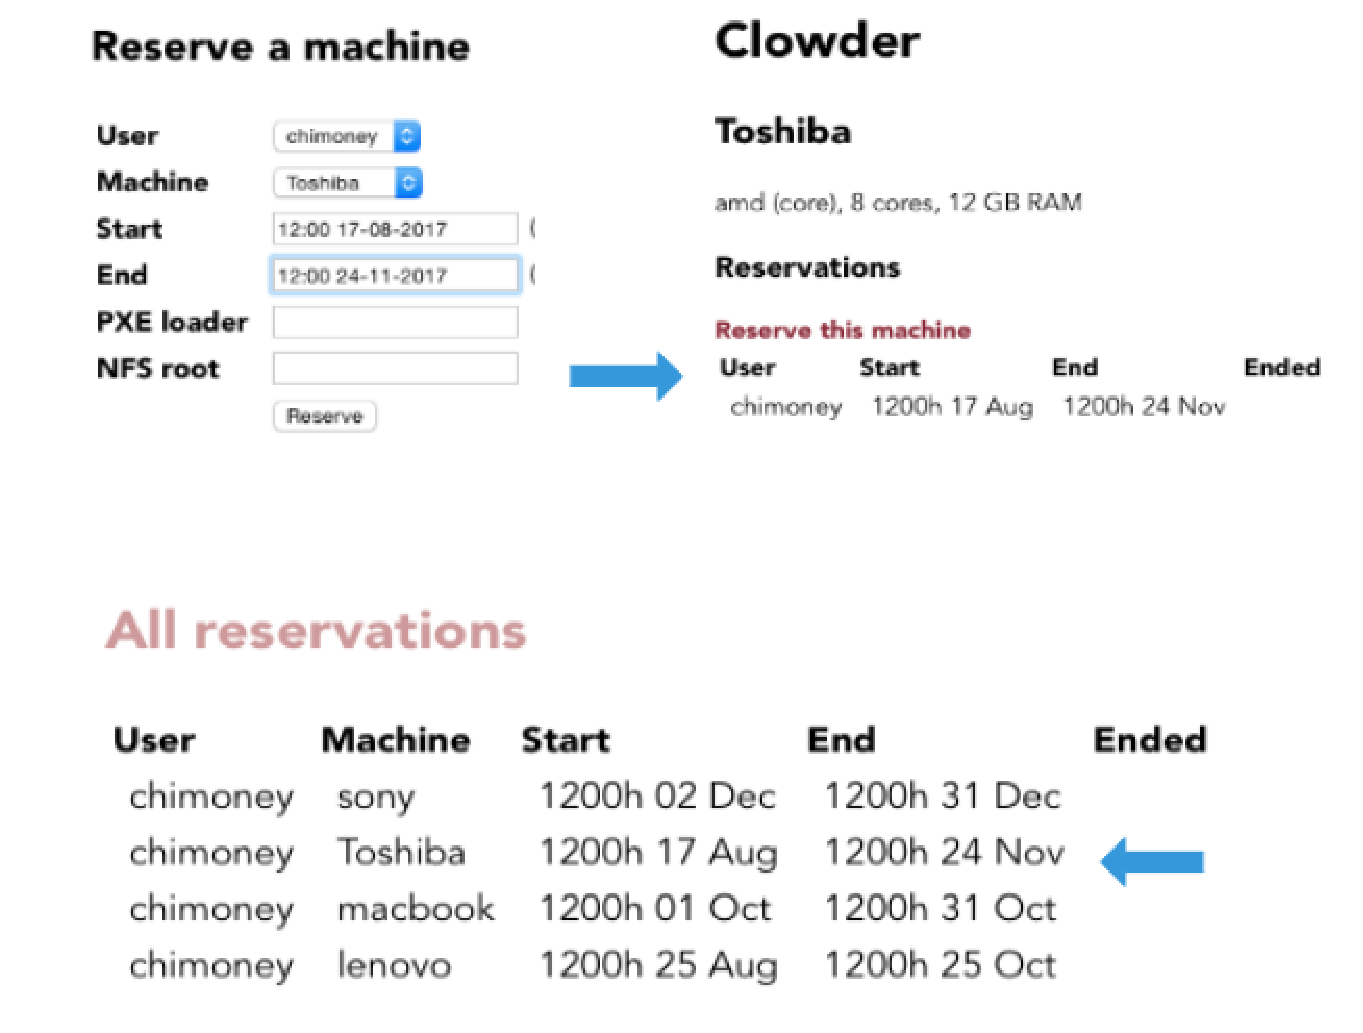
\includegraphics[width=\linewidth]{reserve.eps}
  \label{fig:reserve}
  \caption{Reservation function}
\end{figure}

\section*{Updating a machine}
Update functionality allow users to change the details of a machine already stored in the database. This is to enable them update the information about each machine as needed when ever there is an upgrade in the system. We have tested this functionality by changing the entire information of a machine listed in the inventory. Figure \ref{fig:reserve}  shows an example of this test case.

\begin{figure}[h]
  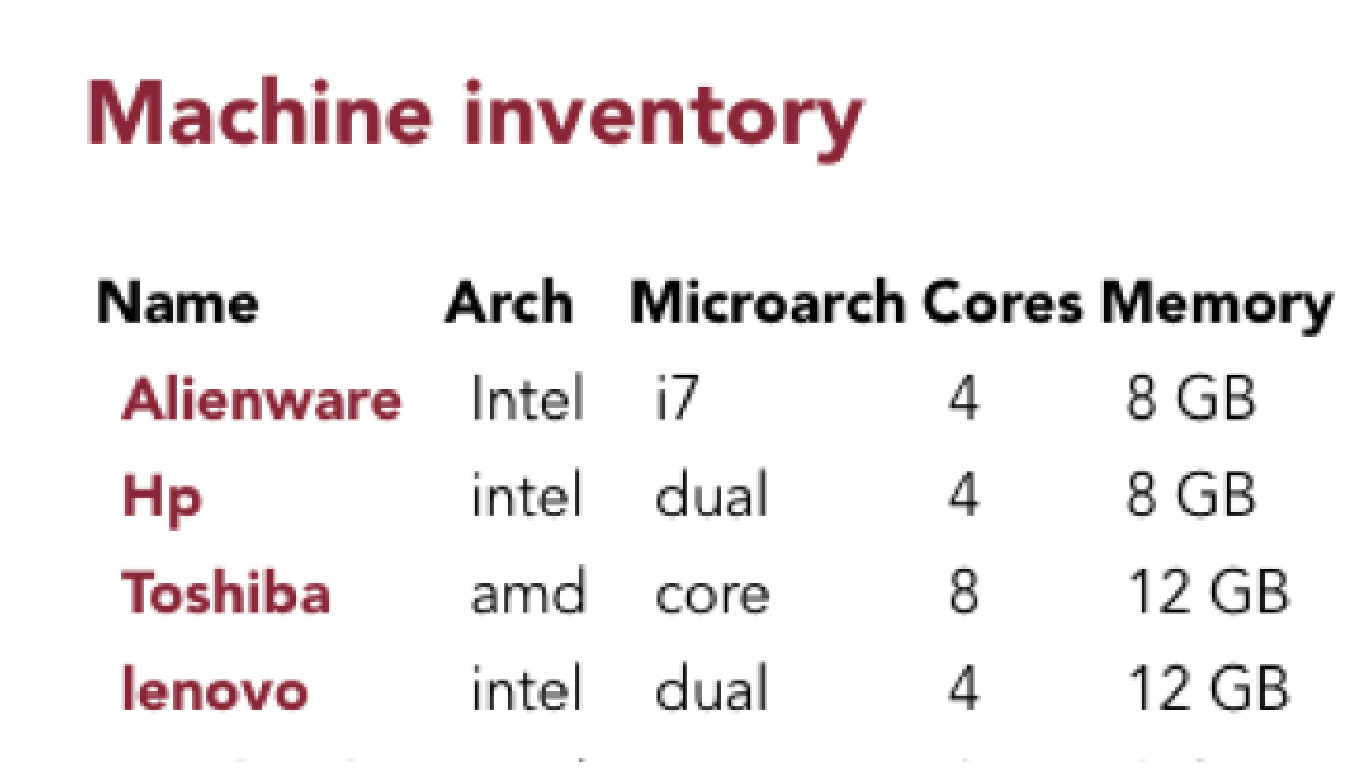
\includegraphics[width=\linewidth]{update.eps}
  \label{fig:reserve}
  \caption{Before update}
\end{figure}


\begin{figure}[h]
  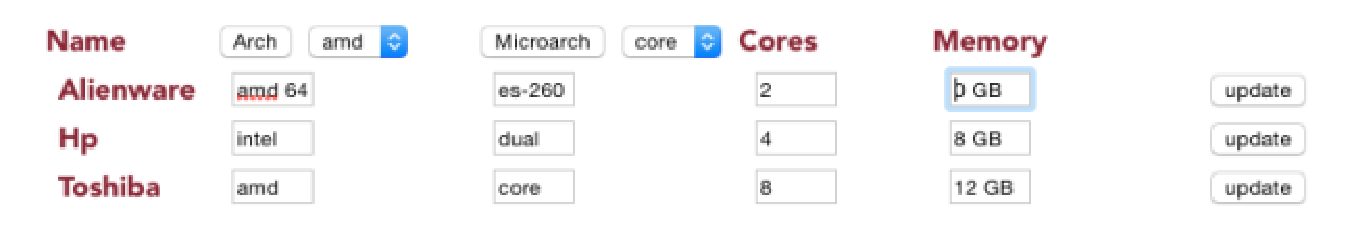
\includegraphics[width=\linewidth]{change.eps}
  \label{fig:reserve}
  \caption{Editing machine details}
\end{figure}

\begin{figure}[h]
  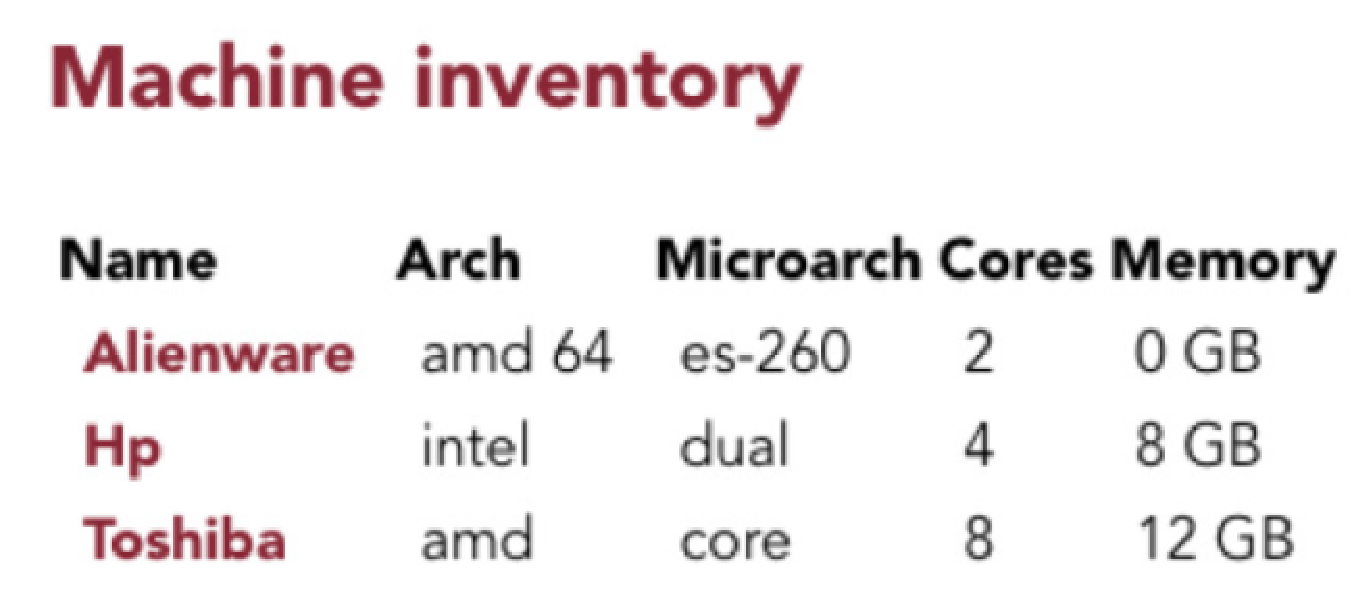
\includegraphics[width=\linewidth]{update2.eps}
  \label{fig:reserve}
  \caption{Updated machine properties}
\end{figure}
\pagebreak

\section*{filtering inventory}
This functionality helps user to filter the inventory using the context of desired information. User is able to filter the machines inventory with memory size. The size range is inserted in the search to get the list of machines that fall within the range. When the button is clicked, the  server returns the list of machine that falls in the range. Another type of filtering is the the drop list filter. This type has a dropdown menu user select a context option to search for. For exaple, user can filter the machine inventory by selecting type os microarchitectre and architect..\begin{figure}[h]
  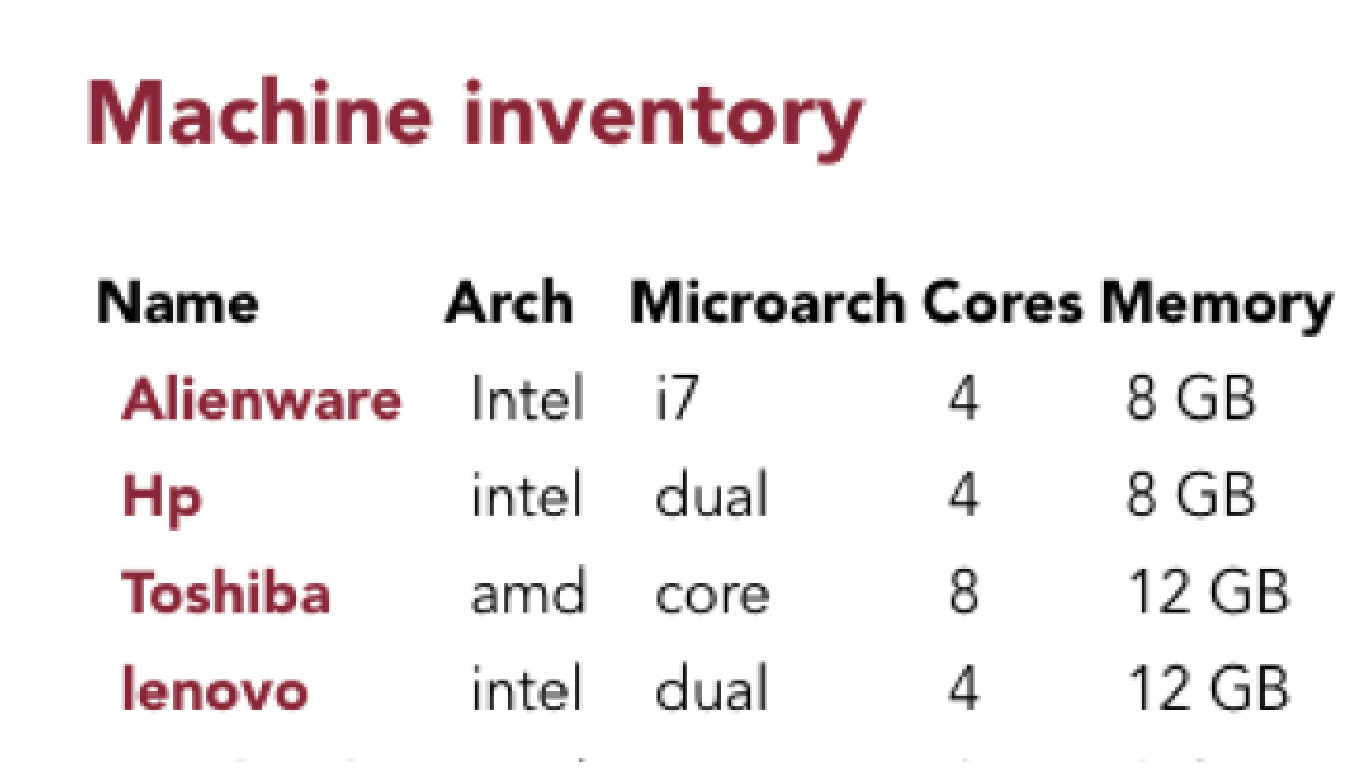
\includegraphics[width=\linewidth]{update.eps}
  \label{fig:reserve}
  \caption{Reservation function}
\end{figure}


\section{Evaluations}


\chapter{Conclusion}
\label{chap:conclusions}

The Clowder system, which was designed to manage test machines, has been improved by addressing the issues of system management and accessibility. It was required to have a flexible user interface for dynamic accessibility, and a functional database system for storage and management. These issues have been resolved by designing a front-end and extending the back-end  software that provides the required functionality on the user interface and the database. We have extended a web interface where users can communicate with the test machines by sending requests via the HTTP protocol. This web interface contains the required functionality for making reservations, updating machine details and viewing the inventory and has generally resolve the issue of user accessibility. Also, as part of the requirement to complete the Clowder system, we extended a SQL database for storing and retrieving data. This database enables the Clowder system to store and manage data of users  activity on the test machines and their information. The database we have created has the ability to plug in a DHCP server which between the Clowder and the test machines. All these components has accomplished the requirement for this project and now made it easier for researchers to use the Clowder system without much complexity. 


\addcontentsline{toc}{chapter}{Bibliography}
\bibliographystyle{ieeetr}
\nocite{*}
\bibliography{ref}

\begin{appendices}
\chapter{Appendix A}
Random generated number of machine and reservations for \autoref{mandr}.
\begin{table}[h!]
  \label{tab:Scattered plot data}
  \begin{tabular}{l|c||r}
    No & Number of Machines & Number of Reservations\\
    \hline
    1 &5 &10  \\
    2 &10 &5 \\
    3 & 15&550  \\
    4 & 20&35  \\
    5 & 50&180  \\
    6 &100 &670 \\
    7&150&120 \\
    8&250&1000 \\
    9&500&50 \\
    10&1000&180 \\
    11&2000&1600 \\
  \end{tabular}
  \caption{Scattered plot data}
\end{table}

The following table shows the data generated from Network and Layout time of the software performance as  shown in \autoref{available}, \autoref{addmachine} and \autoref{addreservation}.
\begin{table}[h!]
\label{tab:availabledata}
\begin{tabular}{l|c||r}
No of Machines & Network Time(ms) & Layout Time(ms)\\
\hline
30&85&35 \\
65&180&65 \\
125&420&180 \\
250&991&248 \\
500&3100&460 \\
1000&9000&860 \\
2000&18000&1680 \\ 
\end{tabular}
\end{table}

\begin{table}[h!]
\label{tab:availabledata}
\begin{tabular}{l|c||r}
No of Machines & Network Time(ms) & layout Time(ms)\\
\hline
30&62&25 \\
65&134&43 \\
125&280&80 \\
250&571&170 \\
500&1000&380 \\
1000&1700&810 \\
2000&2550&1800 \\ 
\end{tabular}
\end{table}

\begin{table}[h!]
\label{tab:availabledata}
\begin{tabular}{l|c||r}
No of Machines & Network Time(ms)& Layout Time(ms)\\
\hline
30&147&37 \\
65&231&52 \\
125&445&74 \\
250&870&120 \\
500&1300&340 \\
1000&2800&447 \\
2000&3960&830 \\ 
\end{tabular}
\end{table}
\end{appendices}

% If you have no appendices, remove the following two lines.
% If you have more appdences, add them as necessary.
\appendix
\chapter{Appendix title}
\label{apdx:somelabel}
This is Appendix~\ref{apdx:somelabel}.

\end{document}